\documentclass{article}
\usepackage{tikz}
\begin{document}
\begin{figure}[!h]
	\centering
	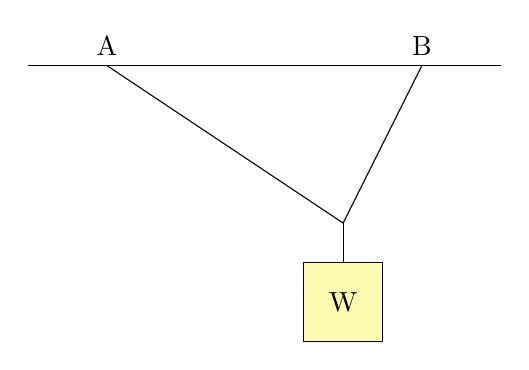
\begin{tikzpicture}
		\coordinate (A) at (1,4);
		\coordinate (B) at (5,4);
		\coordinate (C) at (4,2);
		\coordinate (D) at (4,1.5);
		\coordinate (E) at (0,4);
		\coordinate (F) at (6,4);
		\coordinate (G) at (4,1);
		\draw (E) -- (F);
		\draw (A) -- (C);
		\draw (A) -- (B);
		\draw (B) -- (C);
		\draw (C) -- (D);
		\draw[draw=black, fill=yellow!30] (3.5,0.5)
			rectangle(4.5,1.5);
		\node at (G){W};
		\node[above] at (A){A};
		\node[above] at (B){B};
	\end{tikzpicture}
	\caption{Example of how to make a graphic}
	\label{}
\end{figure}
\end{document}
